%===================================== CHAP 3 =================================

\chapter{Process and methodology}

\section{Process methodology}

After the initial research on the project and what sort of system to build, the group had difficulties choosing which process model and development methodology to use. The main reason behind this, was that as a part of the initial prestudy phase, the group also looked at existing solutions similar to what the customer had requested. During this, the group found out that more research was required than initially assumed. It became apparent that an application existed that satisfied two of the requirements specified by the customer, as well as some other supported protocols. The option of expanding this product arose, and the group realized it would have a large impact on the project. Both the quality of the code, and the degree of requirements achieved would be affected in a positive way.

The project was split into two different phases. The first phase, would take shape as a research project, using models and techniques relevant to performing a research project. The secondary phase would be dependant on the outcome of the research phase. During our exploration of the existing solution, it became apparent that an iterative, incremental development process was suitable for both outcomes. Detailed description of the methodologies, models and techniques used are explained in their respective sections below.

\subsection{Research}

The research methodology chosen was a modified version of the phase-gate model\footnote{\url{http://en.wikipedia.org/wiki/Phase-gate_model}}. The model was chosen due the need of a structured way of performing research, as none of the group members had much experience with such work. After considering some different ways of structuring it, the phase-gate model was chosen as the most suitable. This is a model made for research and product prototyping work. The model describes a time period as a phase. Furthermore, each phase has a gate, which is a goal or evaluation criteria that has to be met. In this case, each phase was a part of the research required, in order to choose whether or not to further develop Apollo. The traditional model commonly has five such phases, whereas the groups usage of the model can be viewed as the discovery and scope phases. Further phases of the model were not executed. Individually, each group member used these first phases as a research cycle, where they discovered new aspects or possible problems. After evaluating whether or not it would be technically and time-wise achievable for the group, further and deeper research proceeded. If an aspect or problem that would not pass the gate evaluation criteria appeared, further research would be aborted and the alternative development plan executed.

Instead of researching each task in succession, the tasks were done in parallel. This was accomplished by distributing them among the group members. The gates of the research phase, was to reach a decision on whether or not the different aspects of further development of Apollo was doable. The evaluation criteria had to yield a positive result, in order to proceed with Apollo.

At the end of the phase, a final decision had to be made. This was due to time constraints, and the fact that development work had to begin. At the end of the research phase, the group would cooperatively assess the research done. The plan was for each group member to present the research work done, and argue for whether or not the group had sufficient knowledge to proceed. A final decision was made after cooperatively assessing all the aspects.

\begin{center}
  \begin{figure}[ht!]
    \makebox[\textwidth]{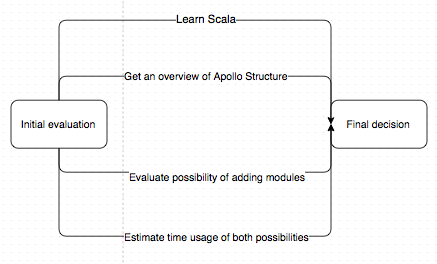
\includegraphics[width=\textwidth]{fig/PhaseGate.png}}
    \caption{Model of the research work}
    \label{fig:phasegate}
  \end{figure}
\end{center}

\subsection{Development}

The second phase would incorporate an iterative and incremental development methodology, with addition of elements from Test Driven Development (TDD). In any case, these were suitable models. Partially because the planning and research were done beforehand, and partially due to the fact that it was a development project.

Scrum\footnote{\url{http://no.wikipedia.org/wiki/Scrum}} was chosen as the agile development method of choice. In contrast to the traditional waterfall model, Scrum is a methodology based on incrementally developing a product. It also defines iterations, called sprints in Scrum. With each sprint, a new increment of the product is delivered. Additionally, the group incorporated scrum meetings, where each group member gave a quick summary of the work done and problems encountered. At the end of each sprint, the group had a longer meeting, in order to evaluate to which degree the planned tasks were completed. A detailed plan of the next sprint was also formed.

All the group members had prior experience with this model from previous projects. Additionally, Scrum was suited for this project due to the fact that it provides frequent updates from all of the members. This was important to keep track of progress, as well as planning customer and supervisor meetings. More generally, using Scrum allowed the group to react to changes in requirements, either due to problems arising, time constraints or alterations made by the customer.

Elements from Test Driven Development were planned to be used in suitable parts of the development process, mainly models and methods with a high degree of logical operations. At times when a task had clear testing conditions, tests were written before the actual program code. Tasks were considered completed, once they had passed all the tests. However, due to the complexity of the system, and discovery of new problems and solutions to these problems, behaviour of methods changed. This prompted us to adjust the tests after modifications of the methods were performed.

\subsection{Report}

The report was a big factor when considering resource management in the project. Thus, a structured way of writing the report was required. The group used different methods to make sure that the report was up to date. All decisions or goals met were noted in the report. The notes in the report were then elaborated upon by all the group members, to create meaningful sections. Additionally, all new major changes to the report were reviewed by all the members, before they were finally agreed upon.

Design was also a factor when creating the report. The decision to use Latex was partially made due to this. Additionally, it was important to make figures and tables as understandable as possible. The general strategy used to achieve this was to have group members, as well as the supervisor give feedback.

Before the delivery deadline of each version of the report, the group set time aside for review and discussion. This phase also included consideration of the feedback received from the supervisor and customer. After all input and feedback were considered, a final version was cooperatively written and agreed upon.

To ensure the quality of the language and readability, a third party with good English language skills was involved to read and comment the report.

\section{Project Organization}

After discussing with the customer, the team decided to have iterations lasting two weeks, starting Monday 26 of January. The two weeks gave the group room to plan according to mandatory work in other courses. The customer also recommended and preferred having weekly meetings. However, due to the extended research phase, the start of the first development cycle was moved.

Furthermore, a distribution of roles was made. This was mainly based on the previous experience of each member. However, it was also important to cover the most common roles in software development teams\footnote{\url{http://zimmer.csufresno.edu/~sasanr/Teaching-Material/SAD/breaking down software development roles.pdf}}, and to cover most of the phases in the systems development life cycle (SDLC)\footnote{\url{http://en.wikipedia.org/wiki/Systems_development_life_cycle}}. Since the group only consisted of six people, it was important to declare these roles, to prevent some aspects of the development life cycle to be neglected.

\subsection{Product owner}

The product owners were Frank T. Johnsen and Trude H. Bloebaum from FFI. Johnsen was responsible for communication with the development team, and also had the responsibility for providing the group feedback about the product. Other than providing requirements and defining the scope of the project, the customer did not participate in any development.

\subsection{Scrum master}

Walleraunet was given the role of scrum master. This was due to him having prior acquaintance with the customer, as well as prior experience in the role. A scrum master has the main responsibility for monitoring progress and deliverables, as well as being the main communication link between the team and the customer.

\subsection{Scrum team}

The other five members of the group constituted  the development team. The team and the scrum master was responsible for developing the product, as well as completing the other deliverables in time. In order to distribute some responsibility away from the Scrum master, the group assigned members to different areas of the project. The group created roles for the remaining five members of the group. The goal was for these roles to cover all the aspects of the project. That meant that if any issues arose, one would always have someone to consult. Additionally, roles were distributed in order to complement the skills of each member.

\subsubsection{Lead developer}

The lead developer's role was keeping control of the progress of the development part of the project. The role were given to Skraastad due to his experience and knowledge of the development tools and environment. Keeping track of inter-sprint progress, version control, development planning and integration were key responsibilities of the lead developer. Additionally, the lead developer would be the link between the solutions architecture and the rest of the development team, providing more detailed descriptions and structure of the different system components.

\subsubsection{Report and documentation}

Berg was responsible for distributing work regarding the report and documentation writing. The main task of Berg was documenting work to be included in the report, and ensuring progress. He was also responsible for making sure that the written documentation was satisfiable.

\subsubsection{Architecture and solutions analysis}

Løvdal was given the responsibility of overseeing the architectural design of the brokering system. He was also responsible for ensuring that all the aspects from the functional analysis was mapped into respective implementable technical solutions.

\subsubsection{Testing and configuration management}

Due to the nature of the project description, the group's choice of architecture, and the complexity of the final system, testing and configuration management was very important. To ensure that none of the relevant aspects of unit, integration and system testing were neglected, Dalby was given these responsibilities. Proper configuration of the systems, and ensuring that testing of different configurations and settings were thoroughly executed, were his main tasks.

\subsubsection{Design, user experience and functional analysis}

One of the main features of the system was the administration interface, with the ability to perform topic mapping and administer the configuration. To ensure that this part of the system was informative and intuitive, Tørnvall was given the responsibility to oversee the part of the system, with emphasis on interface design and user experience. Additionally, he was responsible for expanding on the overall requirements given by the customer, refining them and exploring functional dependencies. This to ensure that the requirements were as precise, clear and complete as possible, reducing the risk of neglecting potential aspects of the system functionality.

\clearpage

\section{Resource management}

The following describes plans for distribution of time and manpower. They are meant to provide a simple visualization of the work planned, as well as tools to track progress. The resource distribution work started in the introduction phase of the project, and was completed after deciding on the project methodology.

\subsection{Work breakdown}

The work breakdown structure(WBS) provides an overview of the different work packages the project is divided into. It is designed as an hierarchy, where each package may have several sub-packages. It also provides a plan for time usage on each major package. The WBS was used as a tool to create the gannt diagram.

\begin{center}
  \begin{figure}[ht!]
    \makebox[\textwidth]{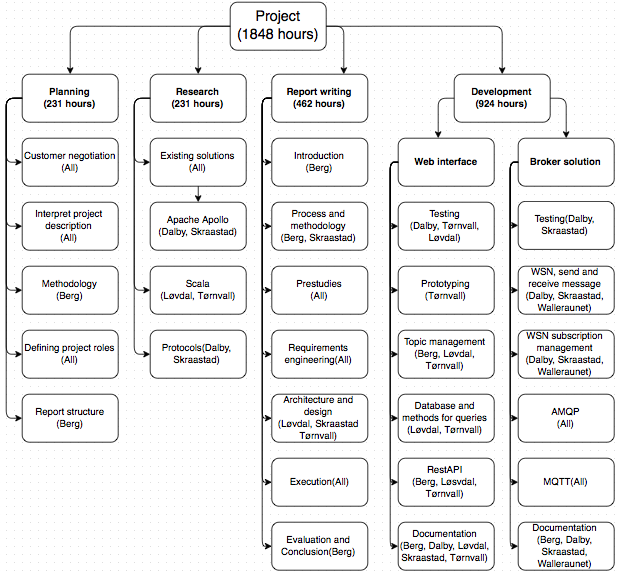
\includegraphics[width=\textwidth]{fig/WBS.png}}
    \caption{Work breakdown structure}
    \label{fig:Work breakdown structure}
  \end{figure}
\end{center}

\begin{center}
  \begin{figure}[ht!]
    \makebox[\textwidth]{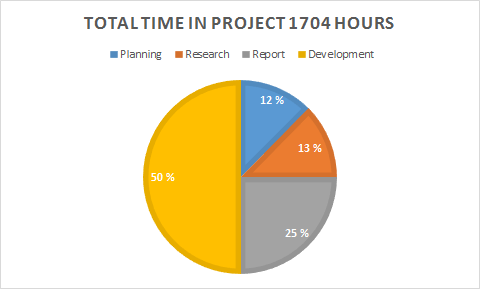
\includegraphics[width=\textwidth]{fig/kakediagram.png}}
    \caption{Main packet structure in percent}
    \label{fig:Main structure diagram}
  \end{figure}
\end{center}

\subsection{Gantt diagram}

Following is the gantt diagram for the project. The goal of this figure is to provide a simple overview of the planned time-distribution of each task in the project. The chart consists of the work packages from the WBS, which has been distributed over the different sprints. This was done in order to make a schedule. Note that unit testing and meetings with the supervisor and customer are not included. They happened during every sprint, and was incorporated in the schedule.

\begin{center}
  \begin{figure}[ht!]
    \makebox[\textwidth]{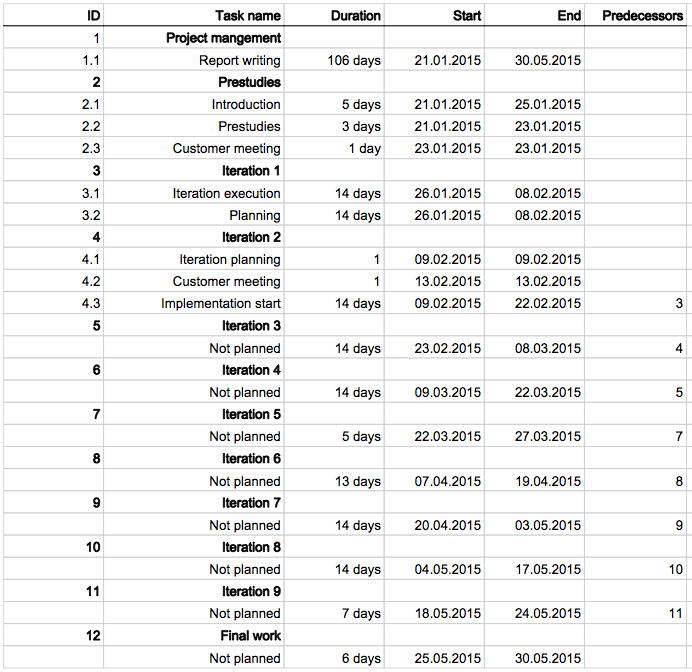
\includegraphics[width=0.75\textwidth]{fig/Gantt.png}}
    \caption{Gantt diagram}
    \label{fig:gantt}
  \end{figure}
\end{center}

\clearpage

\subsection{Available time}

Below is a table showing the time available to us. This was meant as a supplement to the gannt diagram, providing a simple overview of the planned time usage. It accounts for Easter, as well as other holidays.

\begin{table}[h]
\centering
\begin{minipage}{\textwidth}
\resizebox{\textwidth}{!}{%
\begin{tabular}{|p{0.3\linewidth}
                |p{0.2\linewidth}
                |p{0.2\linewidth}
                |p{0.15\linewidth}
                |p{0.15\linewidth}|}
\hline
\textbf{Task}                        & \textbf{Start}         & \textbf{End}           & \textbf{Duration}      & \textbf{Hours}     \\ \hline
Planning and research phase & 21/01/2015    & 24/02/2015    & 14 days       & 336 hours \\ \hline
Iteration 1                 & 25/02/2015    & 06/03/2015    & 8 days        & 192 hours \\ \hline
Iteration 2                 & 09/03/2015    & 20/03/2015    & 10 days       & 240 hours \\ \hline
Iteration 3                 & 23/03/2015    & 01/04/2015    & 8 days        & 96 hours \footnote{Easter holiday and adjusted for the leave of abcence of three group members (USA)}  \\ \hline
Iteration 4                 & 07/04/2015    & 17/04/2015    & 9 days        & 216 hours \footnote{Monday of Orthodox Easter} \\ \hline
Iteration 5                 & 20/04/2015    & 30/04/2015    & 9 days        & 216 hours \footnote{First of May} \\ \hline
Iteration 6                 & 04/05/2015    & 15/05/2015    & 9 days        & 216 hours \footnote{Ascension Day} \\ \hline
Iteration 7                 & 18/05/2015    & 30/05/2015    & 10 days       & 240 hours \\ \hline
\textbf{Total}              &               &               & \textbf{77 days} & \textbf{1752 days} \\ \hline  
\end{tabular}
}
\end{minipage}
\caption{Available time}
\label{fig:available_time}
\end{table}